%
% Einleitung zum Skript "uber lineare Algebra
%
% (c) 2012 Prof Dr Andreas Mueller, Hochschule Rapperswil
%
\chapter*{Einleitung}

Die lineare Algebra stellt sich als Grundlage einer grossen
Zahl von Theorien heraus.
Aufgabe dieser Vorlesung ist, die
Grundlagen dieser Theorie sowie die wichtigsten Anwendungsthemen
zu vermitteln.
Um die Darstellung der Theorie nicht zu stark zu unterbrechen,
werden gr"osser Anwendungen in separaten Abschnitten am Ende
jedes Kapitels beschrieben.

\section*{Behandelte Themen}
\subsection*{Kapitel 1: Lineare Gleichungssysteme}
Die Lineare Algebra besch"aftigt sich zun"achst mit der L"osung linearer
Gleichungen.
Dazu werden im ersten Kapitel einige Methoden bereitgestellt,
und es wird diskutiert, unter welchen Voraussetzungen ein
Gleichungssystem keine, genau eine oder unendlich viele
L"osungen hat.
Die Techniken motivieren auch einen neuen Kalk"ul, die Matrizenrechnung,
welcher das Rechnen mit Zahlen und Vektoren, das vielen
Studierenden bereits bekannt ist, auf beliebige Dimensionen erweitert,
und zudem ein Produkt einf"uhrt.

\subsection*{Kapitel 2: Determinanten}
F"ur Gleichungssysteme mit gleich vielen Gleichungen wie Unbekannten
kann man ein Art Kennzahl finden, welche direkt Aussagen kann,
ob ein Gleichungssystem eine eindeutige L"osung hat.
Erstaunlicherweise ist die so definierte Gr"osse, die Determinante,
noch viel universeller.
Man kann damit auch direkt ein Gleichungssystem l"osen, oder
die inverse Matrix berechnen.
Ausserdem l"asst sich die Determinante zur Fl"achen- und Volumenberechnung
verwenden, und man kann damit das Vektorprodukt definieren.

\subsection*{Kapitel 3: Vektorgeometrie}
Die abstrakte Sprache der Vektoren kann auf die Geometrie angewendet
werden.
L"osungen geometrischer Aufgaben werden damit berechnbar,
meistens als L"osungen lineare Gleichungsysteme.

\subsection*{Kapitel 4: Lineare R"aume}
Die Lineare Algebra ist besonders gut auf spezielle
Teilmengen des Raumes adaptiert, n"amlich Geraden,
Ebenen oder h"oherdimensionale Analoga.

\subsection*{Kapitel 5: Matrixzerlegungen}
Der Gauss-Algorithmus aus Kapitel~1 kann auch als eine
Zerlegung einer Matrix in zwei Dreiecksmatrizen formuliert werden.
Es lassen sich ber auch andere Zerlegungen finden, die je
nach Anwendungsfall geeigneter sind.

\subsection*{Kapitel 6: Eigenwerte und Eigenvektoren}
Das wahrscheinlich wichtigste Problem der lineare Algebra
ist das Eigenwertproblem.
Dieses Kapitel beschreibt das Problem und die L"osung mit Hilfe
des charakteristischen Polynoms.
In einem eigenen Abschnitt werden ausserdem numerische Algorithmen
beschrieben, die Eigenwerte und Eigenvektoren auch f"ur gr"ossere
Matrizen finden k"onnen, f"ur welche das charakteristische 
Polynom keinen praktikablen L"osungsweg darstellt.

\section*{Anwendungen}
Jedes Kapitel enth"alt am Ende auch einen Abschnitt mit gr"osseren
Anwendungen der Theorie des Kapitels.

\subsection*{Die Kirchhoffschen Gesetze}
Die Kirchhoffschen Gesetze erlauben die Str"ome in einem Netzwerk
zu berechnen.
Dieses Problem wurde urspr"unglich von Gustav Robert Kirchhoff
formuliert und gel"ost, aber als Nebenresultate seiner Theorie
entstand auch eine ganze Menge von Resultaten "uber Netzwerke,
zum Beispiel zeigt sich, wie man mit Hilfe von Determinanten
die Zahl der m"oglichen Spannb"aume eines Graphen z"ahlen kann.

\subsection*{Kurvenanpassung}
Die Methode der kleinesten Quadrate liefert auch eine Methode,
mit der man zu einer Menge von Messwerten eine bestm"oglich passende
Funktion finden kann.

\subsection*{Wavelets}
Die Orthogonalisierungsmethode erlaubt eine Menge von
Basisfunktionen zu finden, nach denen man eine gesamplete Funktion
besonders effizient entwickeln kann, und deren Weiterentwicklung
zu den Wavelets von grosser praktischer Bedeutung ist.

\subsection*{Google Pagerank}
Suchmaschinen im Internet m"ussen aus einer potentiell sehr grossen Zahl
von Suchresultaten die treffendsten als erste liefern.
Die einzige Quelle zur Bewertung der Resultate kann nur
das Internet selbst sein.

\section*{Die Karte der linearen Algebra}
Die Karte der linearen Algebra auf der folgenden Seite zeigt ein
paar Begriffe, die in den nachfolgenden Kapiteln erkl"art werden.
Der Leser wird aufgefordert, bei Gelegenheit zu dieser Karte
zur"uckzukommen und zu versuchen, ob er den dargestellten
Zusammenh"angen einen Sinn geben kann.

\begin{landscape}
\begin{center}
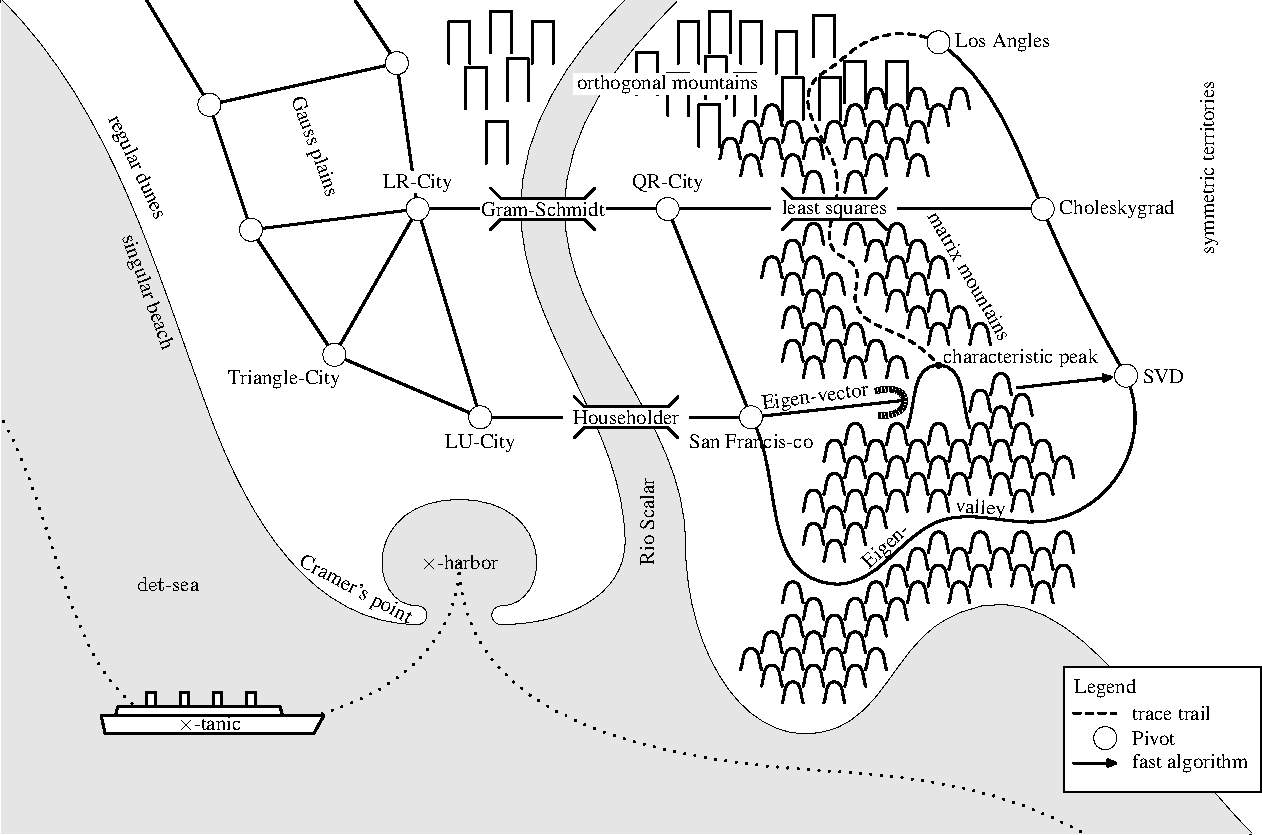
\includegraphics[width=0.95\hsize]{images/linalgmap-1}
\end{center}
\end{landscape}
